\documentclass[conference]{IEEEtran}
\usepackage[english]{babel}
\usepackage[utf8]{inputenc}
\usepackage[T1]{fontenc}
\usepackage{mathtools}
\usepackage{amssymb}
\usepackage{graphicx}

\newcommand{\equref}[1]{Equation~\ref{#1}}
\newcommand{\figref}[1]{Figure~\ref{#1}}
\newcommand{\apref}[1]{Appendix~\ref{#1}}
\newcommand{\secref}[1]{Section~\ref{#1}}
\newcommand{\dindex}[3]{#1_{#2,\;#3}}

\newcommand{\url}[1]{Web address goes here}

\newcommand{\innerimage}[3]{
  \includegraphics[clip=true, trim=#2, width=\linewidth]{assets/#1.pdf}
  \caption{#3}
  \label{fig:#1}
}

\newcommand{\image}[3]{
  \begin{figure}
    \centering
    \innerimage{#1}{#2}{#3}
  \end{figure}
}


\newcommand{\ssdtc}{Steady-State Dynamic Temperature Curve}

\title{Accurate and Fast Steady-State\\Dynamic Temperature Analysis}
\author{Min Bao, Petru Eles, Zebo Peng, and Ivan Ukhov}

\begin{document}
  \maketitle

  \begin{abstract}
    The temperature analysis is one of the most important components of a well-established design of an embedded system. Whenever it is possible, system architects are trying to take it into account in order to produce results of a higher quality in the sense of, for example, reliability and energy consumption. An accurate and fast temperature estimation is not an easy goal to achieve, since the temperature variation is a considerably complicated process that depends on a lot of different parameters, such as the dynamic power consumption and power leakage of the die. The problem becomes much more severe when we make a little step further and put it inside an optimization loop where this type of estimation needs to be performed thousands of times. In this case, the solution should be not only accurate, but also computationally cheap to find. In this paper we propose such a technique that satisfies both criteria, accuracy and speed. Our particular focus of interest is \emph{multiprocessor} system-on-chips that have \emph{periodic} power and, consequently, temperature profiles (for example, the system may execute a periodic application). The proposed solution is analytical, therefore, it is exact from the perspective of the underlying model, also it is fast enough to be used in such search heuristics as the genetic algorithms, that we have chosen to demonstrate our approach.

  \end{abstract}

  \section{Introduction}
  \subsection{Temperature Variation}
Morden policies for prevening temperature runaways and decreasing energy consumption, within such tecniques as dynamic power management (DPM) and dynamic voltage and frequency scaling (DVFS), keep puzzling embedded system architects with a constantly increasing strength. These and similar approaches may cause considerable temperature fluctuations within a multiprocessor system-on-chip (MPSoC), therefore, dramatically decreasing its reliability \cite{mihic2004}, \cite{simunic2005}.

The importance of the temperature distribution over ICs has been widely studied in the literature \cite{lu2004}. Hence, a large number of different methods for performance and energy optimization imposes the maximal temperature constrain. In this essence, the need of fast and accurate methods for obtaining temperature profiles becomes urgent.

In this paper we consider the HotSpot thermal model \cite{huang2006} and propose an extremely fast way to calculate the steady-state dynamic temperature curve (SSDTC) of an embedded system that executes a set of periodic tasks.

In order to demonstrate our approach, we perform the energy optimization with a constrain on the spatial temperature gradient within a die. The constrain is satisfied with the help of SSDTC that delivers the diapason of the temperature fluctuation. The optimization problem is solved through the mapping and scheduling based on genetic algorithms and the list scheduler described in \cite{schmitz2004}.

\subsection{Motivational Example}
TODO.


  \section{Preliminaries}
  The proposed SSDTA technique is based on the well-known RC thermal model that employs the analogy between electrical and thermal circuits. According to this model, the temperature behaviour can be predicted by constracting equivalent RC thermal circuits where electrical current, voltage, resistance, and capacitance are replaced by heat flow, temperature, thermal resistance, and thermal capacitance, correspondingly. The heat equation in this model takes the following matrix form:
\begin{equation} \label{eq:thermal-ode}
  C \frac{dT}{dt} + G T = P
\end{equation}
where $T$ is a vector of temperature, $C$ is the thermal capacitance matrix, $G$ is the thermal conductance matrix (equal to $R^{-1}$, where $R$ is the resistance matrix), and $P$ is a vector of the power dissipation (the source of heat). $C$ and $G$ are $N_n \times N_n$ matrices, $T$ and $P$ are vectors of the length $N_n$, where $N_n$ is the number of thermal nodes. For convenience, in the rest of the paper we use the following denotation:
\begin{equation} \label{eq:initial}
  C \frac{dT}{dt} = A T + B
\end{equation}

An equivalent circuit of a multiprocessor system with a thermal package can be built in a wide range of different ways. Therefore, the number of thermal nodes $N_n$, as well as the conductance and capacitance matrices, depends on a particular realization of the model, i.e., its granularity. For instance, the wide spread thermal simulator HotSpot \cite{huang2006} includes two different implementations, so-called block and grid models. In the block model each core of a multiprocessor system is given one thermal node, while with the grid model the whole die is covered is an adjustable mesh of thermal nodes. Both models have a number of extra nodes for the thermal package of the die which includes the thermal interface material, heat spreader, and heat sink. For example, in case of the block model with $N_p$ processing elements, the total number of thermal nodes can be computed according to the following equation \cite{rao2008}:
\begin{equation} \label{eq:nodes}
  N_n = 4 \times N_p + 12
\end{equation}

The choice of a particular model depends on a desired accuracy. Without loss of generality, we shall use the block model of HotSpot in our experiments.


  \section{Prior Work and Motivation}
  Consider an application with six tasks, denoted ``T0''--``T5'', and a heterogeneous architecture with two cores, labeled ``PE0'' and ``PE1''. The task graph of the application is given in \figref{fig:task-graph} along with the execution times for both cores. The period of the application is 0.06 seconds. A first alternative mapping and schedule, and the resulting SSDTP are shown at the top of \figref{fig:motivation} (where the hight of a task represents its relative dynamic power consumption). It can be observed that initially PE0 is experiencing three thermal cycles. If we change the mapping of T5 and move it to PE1, we achieve two thermal cycles of PE0 instead of three. Finally, if we vary the schedule as well and change the order of T1 and T3, the number of cycles of PE0 becomes one. Using the reliability model from \secref{sec:reliability-model}, we observe improvements in the MTTF of 44.69\% and 54.53\%, respectively, relative to the initial configuration.
\begin{figure}
  \centering
  \subfloat[The task graph.]{
    \label{fig:task-graph}
    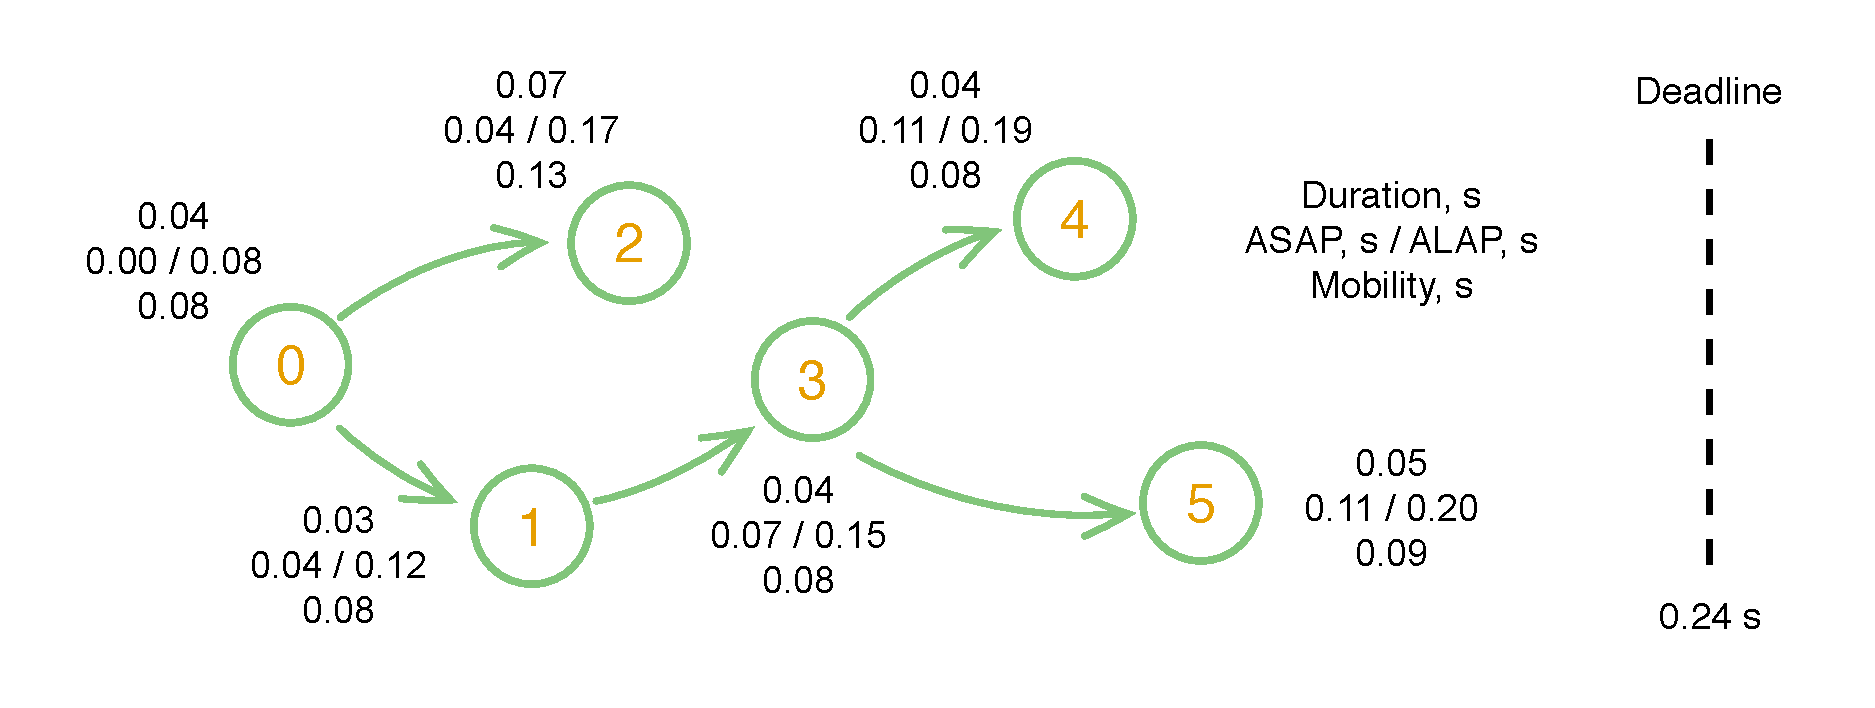
\includegraphics[width=0.8\linewidth]{assets/task-graph.pdf}
  }
  \vspace{-15pt}

  \subfloat[Alternative mappings and schedules.]{
    \label{fig:motivation}
    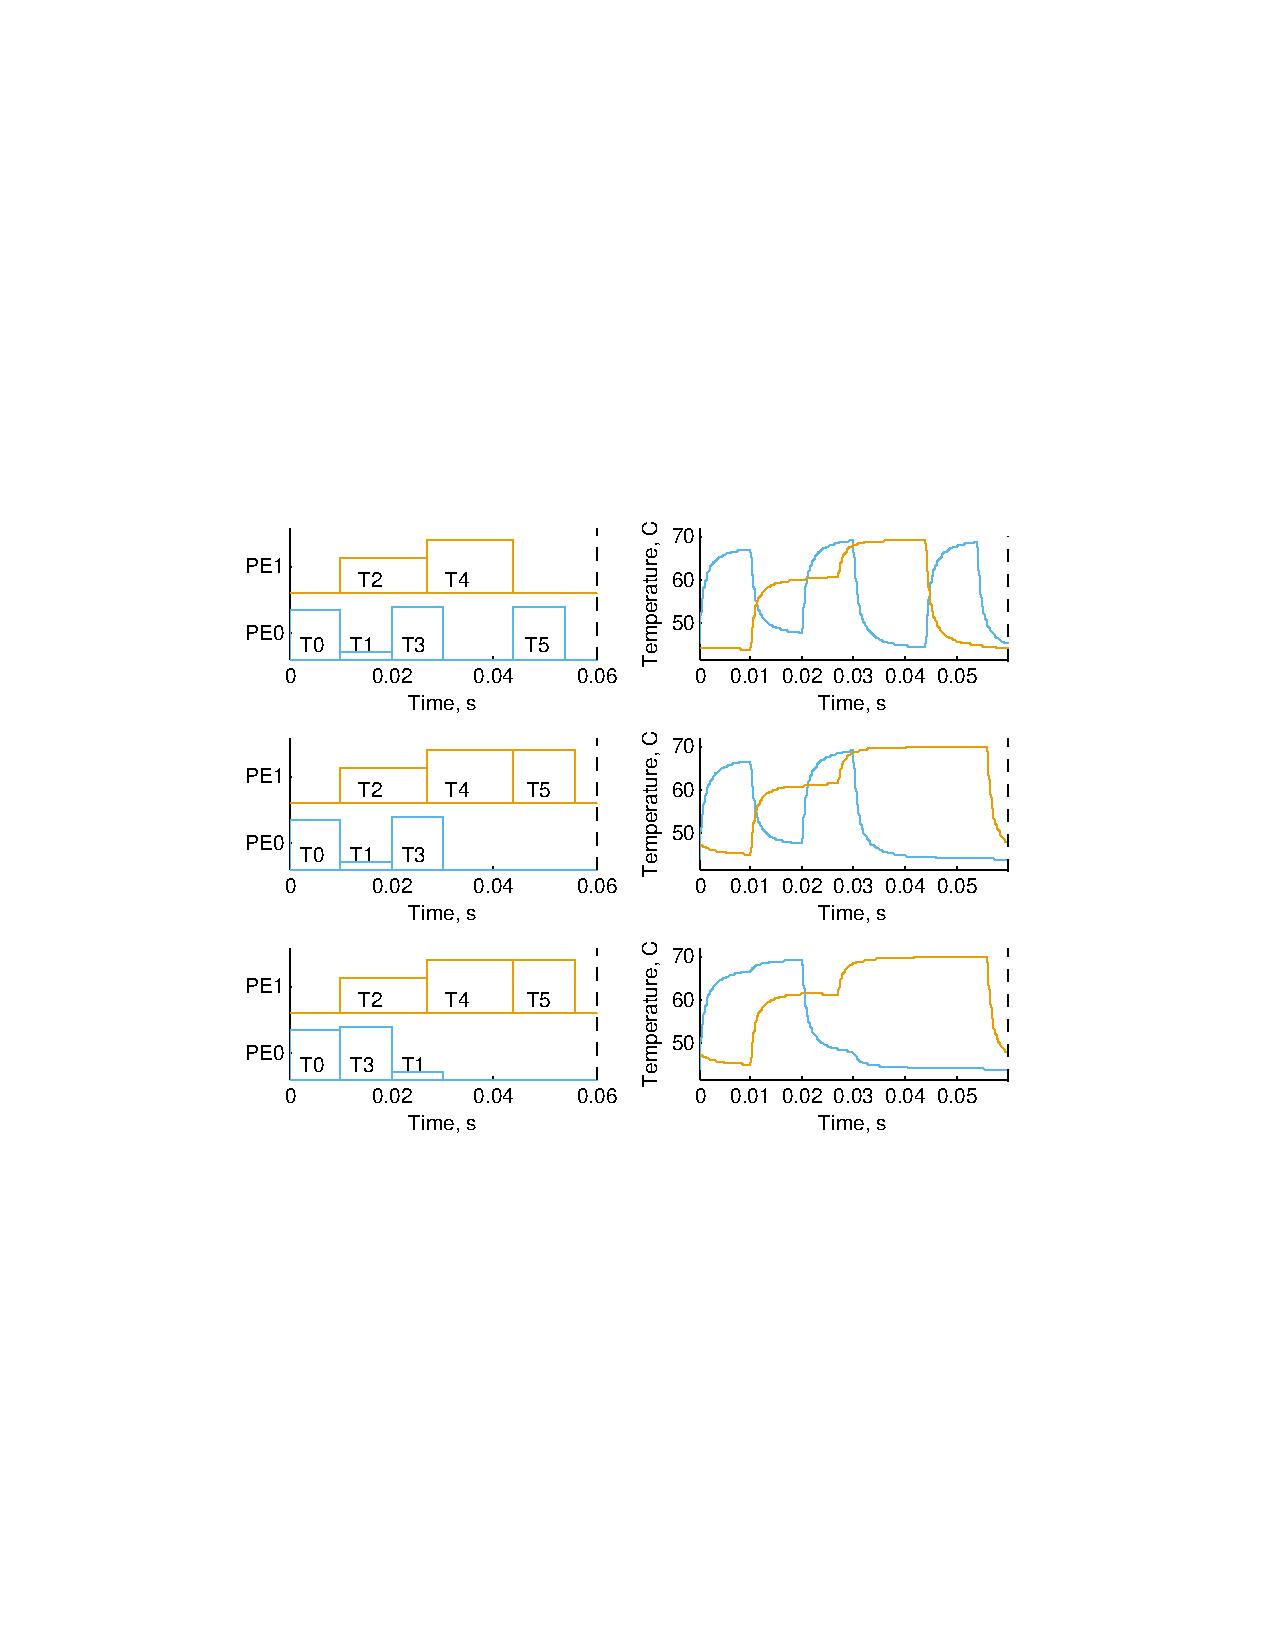
\includegraphics[width=0.8\linewidth]{assets/motivation.pdf}
  }
  \vspace{5pt}
  \caption{Motivational example.}
  \vspace{15pt}
\end{figure}


  \section{Steady-State Dynamic Temperature Profile}
  \subsection{Problem Formulation}
We consider a multiprocessor embedded system that runs a number of periodic tasks. We assume that the power profile of the system is given, and it has periodic nature. Therefore, the overall profile is described with one repeating chunk.

In this case, after the stabilization process, the temperature profile also becomes periodic. This temperature curve is called \ssdtc\ (SSDTC), and our goal is to find it. Furthermore, we want to calculate it quick and accurate enough to be able to use it inside other optimization problems. An example of such problem is given in \secref{sec:results}.

\subsection{Iterative Solution with HotSpot}
One approach to find SSDTC would be to call HotSpot (the tool) with a very long power profile composed of some repeating chunk, but it would take much time to compute (see the comparison in \secref{sec:results}).

\subsection{Direct Analytical Solution}
In order to deal with the problem, we use the analytical approach. First of all, we need to be able to solve \equref{eq:initial} efficiently. The direct solution is:
\begin{equation} \label{eq:solution}
  T(t) = e^{C^{-1}A \cdot t} \cdot T_0 + (C^{-1} \cdot A)^{-1}(e^{C^{-1}A \cdot t} - I)C^{-1} \cdot B
\end{equation}

Here we need to find the matrix exponential of $C^{-1} \cdot A \cdot t$, but it would be easier to do if the matrix were symmetric, because a real symmetric matrix is diagonalizable and has independent (orthogonal) real eigenvectors:
\begin{align}
  & A = U \cdot \Lambda \cdot U^T \label{eq:eigenvalue-decomposition} \\
  & e^A = e^{U \cdot \Lambda \cdot U^T} = U \cdot e^{\Lambda} \cdot U^T \nonumber \\
  & e^{\Lambda} = \left[
      \begin{array}{ccc}
        e^{\lambda_0} & \cdots & 0 \\
        \vdots & \ddots & \vdots \\
        0 & \cdots & e^{\lambda_{n - 1}}
      \end{array}
    \right] \nonumber
\end{align}
where: $A$ is a real symmetric matrix, $U$ is the eigenvectors of $A$, $\Lambda$ is a diagonal matrix of the eigenvalues of $A$ ($\lambda_i$).

Therefore, we want to keep symmetry of the matrix which matrix exponential we are going to compute. In order to achieve this, we do the following substitution:
\begin{align*}
  Y & = C^{\frac{1}{2}} \cdot T \\
  D & = C^{-\frac{1}{2}} \cdot A \cdot C^{-\frac{1}{2}} \\
  E & = C^{-\frac{1}{2}} \cdot B
\end{align*}
with the result:
\begin{align}
  \frac{dY}{dt} & = D \cdot Y + E \nonumber \\
  Y(t) & = e^{D \cdot t} \cdot Y_{0} + D^{-1}(e^{D \cdot t} - I)E \label{eq:modified-solution} \\
  T(t) & = C^{-\frac{1}{2}} \cdot Y(t) \nonumber
\end{align}

Now $D$ is a symmetric matrix, hence, it will be easy to find the matrix exponential of $D \cdot t$ using the eigenvalue decomposition (\equref{eq:eigenvalue-decomposition}):
\[
  e^{D \cdot t} = U \cdot e^{t \cdot \Lambda} \cdot U^T = \left[
      \begin{array}{ccc}
        e^{t \cdot \lambda_0} & \cdots & 0 \\
        \vdots & \ddots & \vdots \\
        0 & \cdots & e^{t \cdot \lambda_{n - 1}}
      \end{array}
    \right]
\]

Each line of the power profile $B$ contains power values for all cores, denoted as $B_i$, at the same period of time $t_i$. Each step of the iterative process we get a vector of temperature values for all cores according to \equref{eq:modified-solution}:
\begin{align}
  & Y_{i+1} = K_i \cdot Y_i + G_i \cdot B_i \label{eq:ce-recurrent} \\
  & K_i = e^{D \cdot t_i} \nonumber \\
  & G_i = D^{-1}(e^{D \cdot t_i} - I) C^{-\frac{1}{2}} \nonumber
\end{align}

Since we perform the eigenvalue decomposition of D (\equref{eq:eigenvalue-decomposition}), $D^{-1}$ can be efficiently computed in the following way:
\[
  D^{-1} = U \cdot \Lambda^{-1} \cdot U^T = U \left[
      \begin{array}{ccc}
        \frac{1}{\lambda_0} & \cdots & 0 \\
        \vdots & \ddots & \vdots \\
        0 & \cdots & \frac{1}{\lambda_{n - 1}}
      \end{array}
    \right] U^T \\
\]
therefore:
\begin{align*}
  G_i & = U \cdot \Lambda^{-1} \cdot U^T (U \cdot e^{t_i \cdot \Lambda} \cdot U^T - U \cdot U^T) C^{-\frac{1}{2}} = \\
      & = U \left[
        \begin{array}{ccc}
          \frac{e^{t_i \cdot \lambda_0} - 1}{\lambda_0} & \cdots & 0 \\
          \vdots & \ddots & \vdots \\
          0 & \cdots & \frac{e^{t_i \cdot \lambda_{n - 1}} - 1}{\lambda_{n - 1}}
        \end{array}
      \right] U^T \cdot C^{-\frac{1}{2}}
\end{align*}

If the time intervals are equal, i.e. the distance in time between two vectors of power values stays the same, the iterative process can be described as the following:
\[
  Y_{i+1} = K \cdot Y_i + G \cdot B_i
\]
where:
\begin{align*}
  & t_i = t_s, \forall i \\
  & K = e^{D \cdot t_s} \\
  & G = D^{-1}(e^{D \cdot t_s}-I) C^{-\frac{1}{2}}
\end{align*}

It should be noted that $K$ and $G$ are constants, since they depend only on the matrices $A$, $C$, and the sampling interval $t_s$.  Both $Y_i$ and $B_i$ are vectors $n \times 1$.

Therefore, in order to find SSDTC, we need to solve the following system of linear equations:
\[
  \begin{cases}
    K_0 \cdot Y_0 - Y_1 & = -Q_0 \\
    ... \\
    K_{m-1} \cdot Y_{m-1} - Y_{m} & = -Q_{m-1}
  \end{cases}
\]
where $Q_i = G_i \cdot B_i$.

Also we have one boundary condition that ensures the temperature to be the same on both sides of the curve:
\begin{equation} \label{eq:boundary-condition}
  Y_0 = Y_m
\end{equation}

Taking it into account, we get:
\[
  \begin{cases}
    K_0 \cdot Y_0 - Y_1 & =-Q_0 \\
    ... \\
    -Y_0 + K_{m-1} \cdot Y_{m-1} & = -Q_{m-1}
  \end{cases}
\]

In this notation, the system can be written as:
\begin{align}
  & AA \cdot YY = BB \label{eq:system} \\
  & AA = \left[
    \begin{array}{ccccc}
      K_0 & -I & 0 & \cdots & 0 \\
      0 & K_1 & -I &  & \vdots \\
      \vdots &  & \ddots & -I & 0 \\
      0 &  &  & K_{m-2} & -I \\
      -I & 0 & \cdots & 0 & K_{m-1}
    \end{array}
  \right] \nonumber \\
  & YY = \left[
    \begin{array}{c}
      Y_0 \\
      Y_1 \\
      \vdots \\
      Y_{m-2} \\
      Y_{m-1}
    \end{array}
  \right] \nonumber \\
  & BB = \left[
    \begin{array}{c}
      -Q_0 \\
      -Q_1 \\
      \vdots \\
      -Q_{m-2} \\
      -Q_{m-1}
    \end{array}
  \right] \nonumber
\end{align}

$AA$ is a square matrix $nm \times nm$. $YY$ and $BB$ are vectors $nm \times 1$. This is the system that can give us desired SSDTC. It should be observed that if the sampling interval is constant, the block diagonal of the matrix $AA$ is composed of the same blocks $K$.

Such systems could be extremely big, therefore, we need to find a fast and accurate way to solve them.

\subsection{Condensed Equation Method}
The system that we have is described with the following recurrent equation:
\begin{equation} \label{eq:recurrent}
  Y_{i + 1} = K_i \cdot Y_i + Q_i, \; i = 0 \dots (m - 1)
\end{equation}

The iterative repetition of this equation leads us to:
\begin{align}
  Y_i & = \prod_{j = 0}^{i - 1} K_j \cdot Y_0 + P_{i - 1}, \; i = 1 \dots m \label{eq:y-recurrent} \\
  P_0 & = Q_0 \nonumber \\
  P_i & = \sum_{l = 1}^i \prod_{j = l}^i K_j \cdot Q_{l - 1} + Q_i, \: i = 1 \dots (m - 1) \nonumber
\end{align}
The last one can be rewritten as:
\begin{equation} \label{eq:p-recurrent}
  P_i = K_i \cdot P_{i - 1} + Q_i, \; i = 1 \dots (m - 1)
\end{equation}

Therefore, we can calculate the final value $Y_m$ from \equref{eq:y-recurrent}:
\[
  Y_m = \prod_{j = 0}^{m - 1} K_j \cdot Y_0 + P_{m - 1}
\]

Taking into account the boundary condition \equref{eq:boundary-condition} and substituting $Y_m$ with $Y_0$, we get the following system of linear equations:
\[
  (I - \prod_{j = 0}^{m - 1} K_j) Y_0 = P_{m - 1}
\]

To solve it, we need to obtain $P_{m - 1}$ from \eqref{eq:p-recurrent}. Once we get $Y_0$, we can use \eqref{eq:recurrent} to get all other vectors $Y_i$.

Now, we know that in case of the fixed sampling interval $K_i = K$. Therefore, the equations become much simpler:
\begin{align}
  & Y_{i + 1} = K \cdot Y_i + Q_i, \; i = 0 \dots (m - 1) \nonumber \\
  & P_i = K \cdot P_{i - 1} + Q_i, \; i = 1 \dots (m - 1) \nonumber \\
  & (I - K^m) Y_0 = P_{m - 1} \label{eq:linear-system}
\end{align}

In this case, $K^m$ can be found very efficiently, since it is a power of the matrix exponential of $D t_s$ (see \equref{eq:ce-recurrent}):
\begin{align*}
  & K = U \cdot e^{\Lambda} \cdot U^T = U \cdot diag(\lambda_0, \dots, \lambda_{n - 1}) \cdot U^T \\
  & K^m = U \cdot e^{\Lambda} \cdot U^T \cdot U e^{\Lambda} \cdot U^T \dots U \cdot e^{\Lambda} \cdot U^T = U \cdot e^{m \Lambda} \cdot U^T
\end{align*}
where $U$ is a matrix of the eigenvectors of $D t_s$ (orthogonal), $\Lambda$ is a diagonal matrix of the eigenvalues of $D t_s$.

Substituting $K^m$ from the last equation into \equref{eq:linear-system}, we get:
\[
  (I - U \cdot e^{m \cdot \Lambda} \cdot U^T) Y_0 = P_{m - 1}
\]

The identity matrix $I$ can be split into $U U^T$, therefore:
\begin{align*}
  & U (I - e^{m \cdot \Lambda}) U^T \cdot Y_0 = P_{m - 1} \\
  & Y_0 = U (I - e^{m \cdot \Lambda})^{-1} U^T \cdot P_{m - 1} \\
  & Y_0 = U \cdot M \cdot U^T \cdot P_{m - 1}
\end{align*}
where $M$ is a diagonal matrix with the following structure:
\[
  M = \left[
    \begin{array}{ccc}
      \frac{1}{1 - e^{m \cdot \lambda_0}} & \cdots & 0 \\
      \vdots & \ddots & \vdots \\
      0 & \cdots & \frac{1}{1 - e^{m \cdot \lambda_{n - 1}}}
    \end{array}
  \right]
\]

As we see, in this approach there is no need to inverse any matrix, the solution of the system is obtained by scalar divisions and a similarity transformation with $U$.

We also can benefit from the matrix exponential in the general case where the time intervals could be different:
\[
  \prod_{j = i}^l K_j = \prod_{j = i}^l e^{D \cdot t_j} = e^{D \sum_{j = i}^l t_j}
\]
since the product of each pair $D \cdot t_j$ and $D \cdot t_k$ is commutative.


  \section{Reliability Model}
  The proposed solution of the steady-state dynamic temperature estimation can be used in a wide range of optimization procedures. One of them is the reliability optimization that we discuss in this section. We perform a temperature-aware task mapping and scheduling in order to address the thermal cycling aging effect while keeping the energy consumption at an appropriate level. Both mapping and scheduling are based on a genetic algorithm \cite{schmitz2004}. Let us start with the overall description of the system.

\subsection{Application Model}
The system executes a periodic application with a set of data-dependent tasks. The overall structure of the application is defined by a task graph:
\begin{align*}
  & G = (\mathcal{V}, \: E, \: \mathcal{T}) \\
  & \mathcal{V} = \{ v_i: \: i = 0 \dots N_t - 1 \}
\end{align*}
where $\mathcal{V}$ is a set of $N_t$ vertices of the graph (tasks), $E$ is a set of edges (data dependencies between tasks), and $\mathcal{T}$ is the period of the application. Each pair of a task $v_i$ and processing element $\pi_j$ is characterized by a tuple $(C_{eff \; ij}, N_{cycles \; ij})$, where $C_{eff \; ij}$ is the effective switched capacitance and $N_{cycles \: ij}$ is the number of clock cycles. These parameters determine the processor load and execution time of the task, respectively.

\subsection{Temperature-Aware Reliability Model} \label{sec:reliability-model}
In the paper we address temperature-driven failure mechanisms with the reliability model presented in \cite{huang2009}, \cite{xiang2010}. The model is based on the assumption that the failure rate has a Weibull distribution (e.g., the thermal cycling, electromigration, etc. \cite{jedec2010}):
\[
  R(t) = e^{-(\frac{t}{\eta})^\beta}
\]
where $\eta$ and $\beta$ are the scaling and shape (slope) parameters, respectively. The mean time to failure (MTTF) for the Weibull distribution is given by the following equation:
\begin{equation} \label{eq:general-mttf}
  MTTF = \eta \; \Gamma(1 + \frac{1}{\beta})
\end{equation}
where $\Gamma$ is the gamma function. The shape parameter is found to be independent on the temperature variation \cite{chang2006}, which is not the case with the scaling parameter $\eta$. Therefore, the distribution can vary from one temperature to another. We can use the same approach as it was shown previously and split the overall period of the application $\mathcal{T}$ into $N_m$ time intervals $\Delta t_i$, so that during each time interval $\Delta t_i$ the corresponding $\eta_i$ is constant and equal to:
\begin{equation} \label{eq:eta-one}
  \eta_i = \frac{MTTF_i}{\Gamma(1 + \frac{1}{\beta})}
\end{equation}
where $MTTF_i$ is the mean time to failure of the $i$th time interval as if we had the failure distribution of this interval all the time. As it was shown in \cite{xiang2010}, the cumulative distribution function can be approximated as the following:
\[
  R(t) = e^{-(\frac{t}{\mathcal{T}} \sum_{i=0}^{N_m - 1} \frac{\Delta t_i}{\eta_i})^\beta}
\]
The formula keeps the form of the Weibull distribution with the scaling parameter equal to:
\begin{equation} \label{eq:eta-many}
  \eta = \frac{\mathcal{T}}{\sum_{i=0}^{N_m - 1} \frac{\Delta t_i}{\eta_i}}
\end{equation}
Consequently, $\eta$ can be substituted into \equref{eq:general-mttf} and the MTTF can be obtained. The only thing that is left is to determine $MTTF_i$ for each of the time intervals. In order to achieve this, we need to focus on the particular failure cause. As it was mentioned previously, the model can handle different failure mechanism; we have chosen the thermal cycling (TC) fatigue where the knowledge of the steady-state temperature in not sufficient and temperature curves should be investigated in details.

The number of thermal cycles to failure can be estimated using a modified version of the well-known Coffin-Manson equation with the Arrhenius term \cite{jedec2010}, \cite{xiang2010}, \cite{ciappa2003}:
\begin{equation} \label{eq:cycles-to-failure}
  \mathcal{N} = A (\Delta T - \Delta T_0)^{-b} e^{\frac{E_a}{k T_{max}}}
\end{equation}
where $A$ is an empirically determined constant, $\Delta T$ is the thermal cycle excursion, $\Delta T_0$ is the portion of the temperature range in the elastic region which does not cause damage, $b$ is the Coffin-Manson exponent with is also empirically determined, $E_{a}$ is the activation energy, $k$ is the Boltzmann constant, and $T_{max}$ is the maximal temperature during the thermal cycle. Having the number of cycles to failure and the duration of one cycle $\Delta t$, we can compute the MTTF that is missing in \equref{eq:eta-one}:
\begin{equation} \label{eq:mttf-cycle}
  MTTF = \mathcal{N} \; \Delta t
\end{equation}
Hence, taking equations \eqref{eq:general-mttf}, \eqref{eq:eta-one}, \eqref{eq:eta-many}, and \eqref{eq:mttf-cycle} together, we obtain the following expression to estimate the MTTF for the whole period of the application:
\begin{align} \label{eq:one-mttf}
  MTTF = \frac{\mathcal{T}}{\sum_{i=0}^{N_m - 1} \frac{1}{\mathcal{N}_i}}
\end{align}

\equref{eq:one-mttf} describes the MTTF of one component, which is a processing element in our case. We assume that each processing element is essential for the proper work of the system, therefore, a failure of any core leads to the total failure of the whole system. Consequently, the MTTF of the system can be estimated as the minimal MTTF among its components:
\begin{align}
  & MTTF_{sys} = \min_{i=0}^{N_p - 1} \; MTTF_i \label{eq:mttf-system} \\
  & MTTF_i = \frac{\mathcal{T}}{\sum_{j=0}^{N_{m \: i} - 1} \frac{1}{\mathcal{N}_{ij}}} \nonumber
\end{align}
where $N_{m \: i}$ is the number of thermal cycles of the $i$th processing element within the application period $\mathcal{T}$ and $\mathcal{N}_{ij}$ is the number of thermal cycles to failure as if the $j$th cycle was being repeated all the time.

\subsection{Motivational Example} \label{sec:motivation}
Consider an application with six tasks, denoted ``T0''--``T5'', and a heterogeneous architecture with two cores, labeled ``PE0'' and ``PE1''. The task graph of the application is given in \figref{fig:task-graph} along with the execution times for both cores. The period of the application is 0.06 seconds. A first alternative mapping and schedule, and the resulting SSDTP are shown at the top of \figref{fig:motivation} (where the hight of a task represents its relative dynamic power consumption). It can be observed that initially PE0 is experiencing three thermal cycles. If we change the mapping of T5 and move it to PE1, we achieve two thermal cycles of PE0 instead of three. Finally, if we vary the schedule as well and change the order of T1 and T3, the number of cycles of PE0 becomes one. Using the reliability model from \secref{sec:reliability-model}, we observe improvements in the MTTF of 44.69\% and 54.53\%, respectively, relative to the initial configuration.
\begin{figure}
  \centering
  \subfloat[The task graph.]{
    \label{fig:task-graph}
    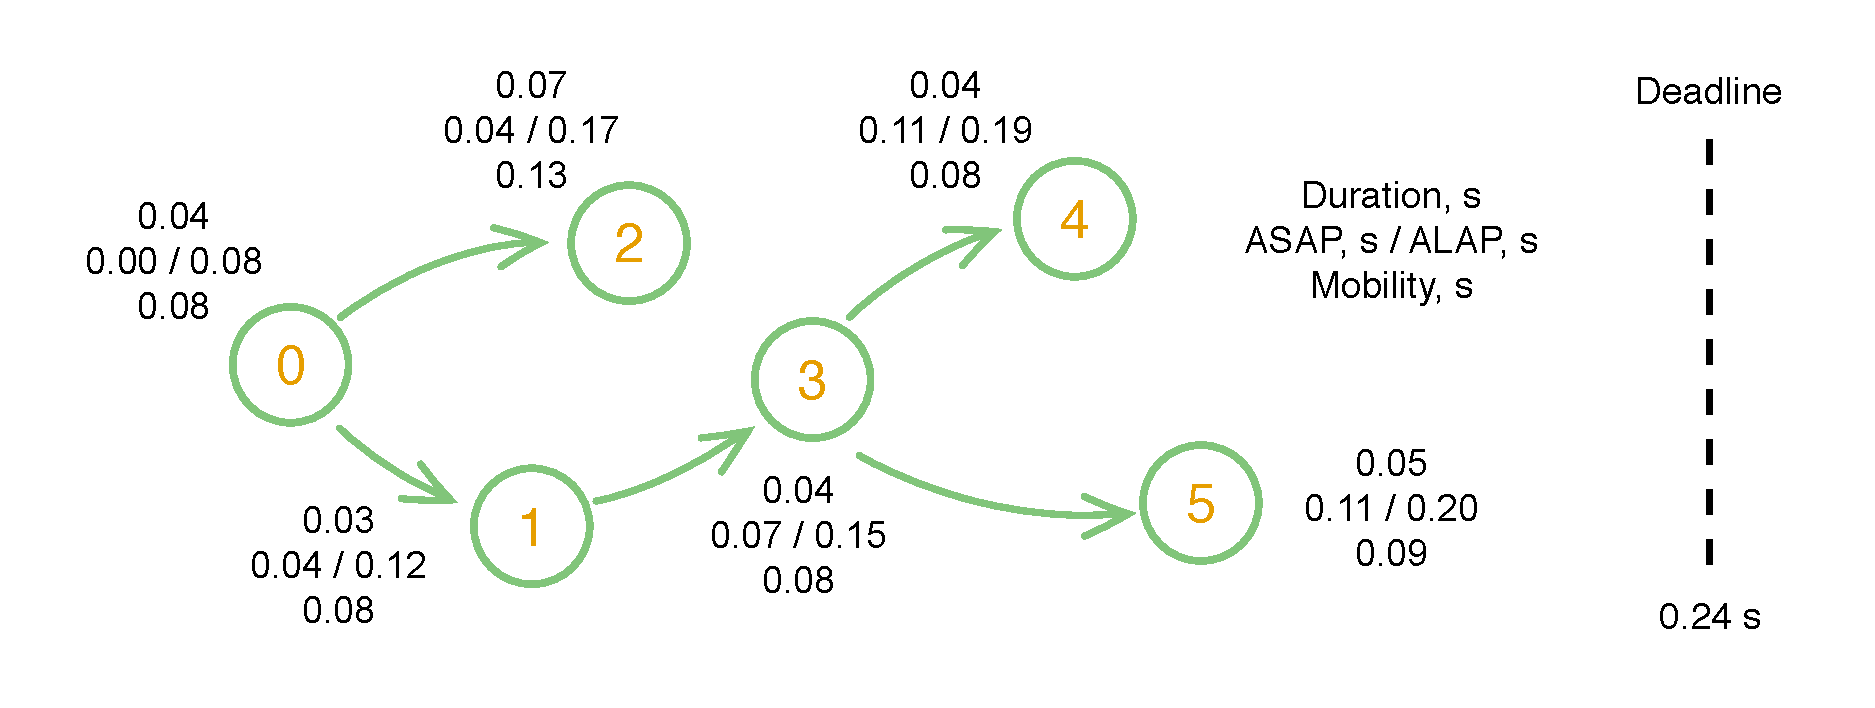
\includegraphics[width=0.8\linewidth]{assets/task-graph.pdf}
  }
  \vspace{-15pt}

  \subfloat[Alternative mappings and schedules.]{
    \label{fig:motivation}
    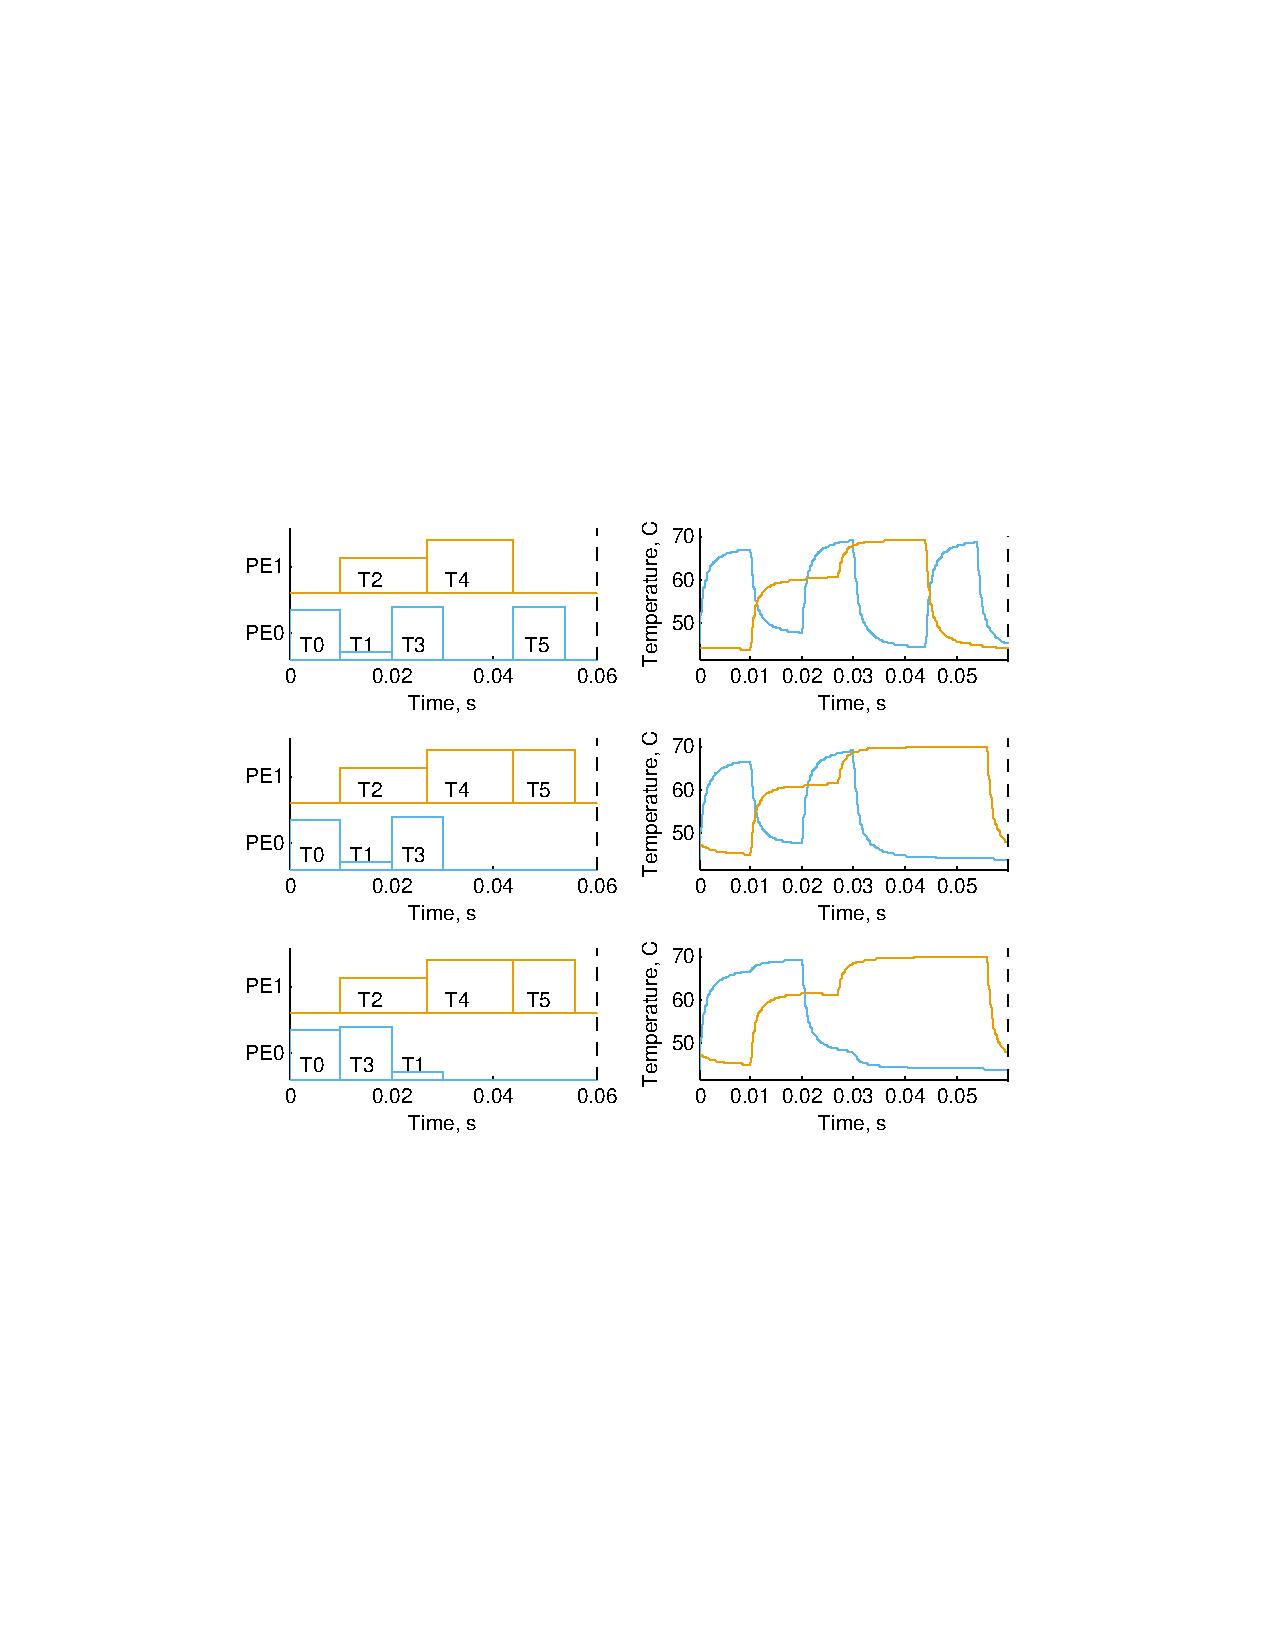
\includegraphics[width=0.8\linewidth]{assets/motivation.pdf}
  }
  \vspace{5pt}
  \caption{Motivational example.}
  \vspace{15pt}
\end{figure}


\subsection{Genetic Algorithm}
The optimization procedure is held by a genetic algorithm (GA) \cite{schmitz2004} that varies mapping and scheduling of the application in order to maximize the MTTF of the system. Each chromosome is a vector of $2 \times N_t$ elements, where the first half encodes priorities of the tasks and the second represents a mapping. The population contains $4 \times N_t$ individuals that are initialized partially randomly and partially based on the mobility of the tasks \cite{schmitz2004}. Each generation, a number of individuals, called parents, are chosen for breeding by the tournament selection with the number of competitors proportional to the population size. The parents undergo the 2-point crossover with $0.8$ probability and uniform mutation with $0.05$ probability. The evolution mechanism follows the elitism model where the best individual always survives. The stopping condition is an absence of improvement within $200$ successive generations.

A chromosome is evaluated in a number of steps. First, the decoded priorities and mapping are given to a list scheduler that produces schedules for each of the cores. If the schedules do not respect the deadline of the application, the solution is penalized proportionally to the delay and is not further evaluated; otherwise, based on the parameters of the architecture and tasks, a dynamic power profile is obtained. Having the dynamic power profile and taking into consideration the leakage power with the linear approximation from \secref{sec:leakage}, the corresponding SSDTP is computed by the CE method. Finally, the SSDTP is assessed in terms of the reliability model given in \equref{eq:mttf-system}, where the rainflow counting method is employed to count thermal cycles \cite{xiang2010}.


  \section{Experimental Results} \label{sec:results}
  \subsection{Computation Performance} \label{sec:results-ssdtp}
In this subsection we investigate the scalability properties of the proposed solution based on the CE method and compare it with one transient temperature simulation (TTS) of the application period, which is not sufficient to reach the SSDTP as it was shown in \secref{sec:hotspot-solution}. To perform the TTA, the HotSpot thermal simulator is used.

\image{scaling-time}{80 230 80 230}{Scalability with the application period for a quad-core architecture. The sampling interval is fixed to 1 millisecond where 1 second on the horizontal axis corresponds to 1000 steps in the power profile. The comparison is given on the semilogarithmic scale.}
\begin{itable}{scaling-time}{|r|r|r|r|r|}
  {Scalability with the application period shown in \figref{fig:scaling-time}.}
  {$\mathcal{T}$ --- the application period, CE --- the Condensed Equation method, TTS --- one Transient Temperature Simulation, NRMSE --- the Normalized Root Mean Square Error.}
  \hline
  $\mathcal{T}$, s & CE, ms & TTS, ms & Speedup, $\times$ & NRMSE, \% \\
  \hline
  \hline
  0.05 &  0.18 &   10.24 & 56.93 & 25.8 \\
   0.1 &  0.35 &   20.26 & 58.30 & 19.0 \\
   0.5 &  1.63 &   97.36 & 59.73 & 9.65 \\
     1 &  3.23 &  193.31 & 59.80 & 7.80 \\
     2 &  6.48 &  382.59 & 59.08 & 6.46 \\
     3 &  9.58 &  573.15 & 59.83 & 5.79 \\
     4 & 12.78 &  770.09 & 60.25 & 5.34 \\
     5 & 16.10 &  964.75 & 59.92 & 5.00 \\
     6 & 19.32 & 1146.87 & 59.36 & 4.72 \\
     7 & 22.51 & 1335.26 & 59.31 & 4.49 \\
     8 & 25.69 & 1536.91 & 59.82 & 4.28 \\
     9 & 28.94 & 1729.39 & 59.76 & 4.09 \\
    10 & 32.65 & 1921.14 & 58.83 & 3.93 \\
  \hline
\end{itable}
First, we vary the application period keeping the sampling interval constant and equal to 1 millisecond. The comparison for a quad-core architecture is given in \figref{fig:scaling-time} and \tabref{tab:scaling-time}. It can be seen that the CE method is roughly 60 times faster than one iteration of the TTA\footnote{All the experiments are done on a Linux machine with Intel\textregistered\ Core\texttrademark\ i7-2600 (3.4GHz, 4 cores, 8 threads) and 8Gb of RAM.}. The application period proportionally corresponds to the number of steps in the power profile (one second is equal to 1000 steps in the power profile in the above-mentioned example). Hence, we would see the same curves, if we were investigating the dependency on the power profile discretization.

\image{scaling-cores}{80 230 80 230}{Scalability with the number of cores. The application period is fixed to 1 second that corresponds to 1000 steps in the power profile. The comparison is given on the semilogarithmic scale.}
\begin{itable}{scaling-cores}{|r|r|r|r|r|}
  {Scalability with the number of cores shown in \figref{fig:scaling-cores}.}
  {$N_p$ --- the number of processing elements (cores), CE --- the Condensed Equation method, TTS --- one Transient Temperature Simulation, NRMSE --- the Normalized Root Mean Square Error.}
  \hline
  $N_p$ & CE, ms & TTS, ms & Speedup, $\times$ & NRMSE, \% \\
  \hline
  \hline
    1 &    0.99 &    97.00 & 97.93 &  25 \\
   10 &   16.46 &   632.50 & 38.44 &  41 \\
   20 &   46.00 &  1761.75 & 38.30 &  69 \\
   30 &   98.49 &  3472.21 & 35.25 & 102 \\
   40 &  172.69 &  5827.77 & 33.75 & 130 \\
   50 &  266.08 &  8771.93 & 32.97 & 142 \\
   60 &  380.95 & 12235.91 & 32.12 & 185 \\
   70 &  517.04 & 16363.54 & 31.65 & 220 \\
   80 &  675.21 & 21104.98 & 31.26 & 245 \\
   90 &  856.20 & 26415.77 & 30.85 & 277 \\
  100 & 1058.35 & 32329.09 & 30.55 & 308 \\
  \hline
\end{itable}
The second part of the comparison is the scalability with the number of processing elements shown in \figref{fig:scaling-cores} and \tabref{tab:scaling-cores}. It can be seen that the difference between computation times of the CE method and one TTS becomes smaller when the number of cores is increasing. At the same time the mismatch between the SSDTP and temperature profile produced by one TTA dramatically increases, which means that larger number of the TTA iterations is required to reach the same level of accuracy.

\subsection{Reliability Optimization}
The experimental setup is the following. Heterogeneous architectures and periodic applications are generated randomly \cite{dick1998} in such a way that the execution time of tasks is uniformly distributed between 1 and 50 milliseconds and the leakage power accounts for 30--55\% of the total power dissipation. The corresponding temperature variation lies between the ambient temperature of $27^{\circ}C$ and maximal temperature of $100^{\circ}C$.

In each of the experiments, we compare the optimized solution with the initial one that is obtained in the following way. First, we calculate the average execution time of each task among the processing elements. Then, we compute the mobility of the tasks and schedule the application according to it \cite{schmitz2004}. The mapping is done along with the scheduling where each task being considered is assigned to the earliest available core in the system. This combination of mapping and scheduling is the starting point for the future optimization. The deadline of the application is set according to the duration of the initial schedule with additional 5\%.

\begin{itable}{mttf-cores}{|r|r|r|r|r|}
  {Reliability optimization for different architectures}
  {$N_p$ --- the number of cores, $N_t$ --- the number of tasks, $t_{avg}$ --- the average computational time, $MTTF_{avg}$ --- the average MTTF improvement, $E_{avg}$ --- the average change in the energy consumption.}
  \hline
  $N_p$ & $N_t$ & $t_{avg}, m$ & $MTTF_{avg}$, \% & $E_{avg}$, \% \\
  \hline
   2 &   20 &   0.66 & 8123.29 & -13.50 \\
   4 &   40 &   2.04 & 7424.04 & -22.92 \\
   8 &   80 &  10.67 & 2819.45 & -21.88 \\
  16 &  160 &  25.38 &  915.11 & -13.78 \\
  32 &  320 &  89.59 &  442.49 &  -8.90 \\
  \hline
\end{itable}
In the first set of experiments, we change the number of cores while keeping the number of tasks per core constant and equal to 10. For each problem we have generated 20 random task graphs of a similar structure and found the average improvement of the MTTF. We also have measured the change in the consumed energy. The results are given in \tabref{tab:mttf-cores}. It can be observed that the temperature-unaware task allocation and scheduling dramatically decrease the lifetime of the device and the optimization based on the SSDTP is a must for an embedded system design framework. Although, the average improvement is decreasing with the growth of the complexity of the problem, it is still considerably high. Note that the energy efficiency of the system is not suffering from the optimization, on the contrary, we observed that the found solutions are generally better with comparison to the initial ones from this perspective.

\begin{itable}{mttf-tasks}{|r|r|r|r|r|}
  {Reliability optimization for different applications}
  {$N_p$ --- the number of cores, $N_t$ --- the number of tasks, $t_{avg}$ --- the average computational time, $MTTF_{avg}$ --- the average MTTF improvement, $E_{avg}$ --- the average change in the energy consumption.}
  \hline
  $N_p$ & $N_t$ & $t_{avg}, m$ & $MTTF_{avg}$, \% & $E_{avg}$, \% \\
  \hline
  4 &  20 & 0.93 & 13029.86 & -26.62 \\
  4 &  40 & 1.81 &  4311.02 & -22.15 \\
  4 &  80 & 0 & 0 & 0 \\
  4 & 160 & 0 & 0 & 0 \\
  4 & 320 & 0 & 0 & 0 \\
  \hline
\end{itable}
For the second set of experiments, we keep the quad-core architecture and vary the number of tasks within the application. The number of randomly generated task graphs per problem is 20. The average improvement of the MTTF along with the change in the energy consumption are given in \tabref{tab:mttf-tasks}. The observations to be made here are similar to the previous ones: taking into consideration the SSDTP of the system during the design stage can significantly prolong the MTTF without sacrificing the energy efficiency of the system.

\begin{itable}{mttf-comparison}{|r|r|r|r|r|}
  {Reliability optimization for different solution techniques}
  {$N_p$ --- the number of cores, $N_t$ --- the number of tasks, $MTTF^{CE}_{avg}$, $MTTF^{TTA}_{avg}$, and $MTTF^{SS}_{avg}$ --- the average improvements of the MTTF obtained by the CE method, TTA with HotSpot, and SS approximation, respectively.}
  \hline
  $N_p$ & $N_t$ & $MTTF^{CE}_{avg}$, \% & $MTTF^{TTA}_{avg}$, \% & $MTTF^{SS}_{avg}$, \% \\
  \hline
  4 &  20 & 0 & 0 & 0 \\
  4 &  40 & 0 & 0 & 0 \\
  4 &  80 & 0 & 0 & 0 \\
  4 & 160 & 0 & 0 & 0 \\
  4 & 320 & 0 & 0 & 0 \\
  \hline
\end{itable}
Finally, we compare the results of the optimization delivered by the CE method, TTA with HotSpot, and steady-state approximation (SS) discussed in \secref{sec:steady-state-approximation} for the same setup as in the previous set of experiments with the fixed architecture. The final solution found by the later two methods, TTA and SS, are reevaluated using the CE method and compared with the solutions found only by the CE approach. The results are summarized in \tabref{tab:mttf-comparison}. \todo{Obtain results and discuss.}


  \section{Conclusion}
  The SSDTA is an essential part of the embedded system design. In this paper we formutated the problem and proposed an elegant anlytical technique to solve it. The solution is both accurate and fast enough to be a decent tool of the designer. Using the proposed approach, we conducted a temperature-aware reliability optimization based on the thermal cycling failure mechanism and shown that taking into consideration the temperature variations within a multicore platform can significantly prolong its lifetime without affecting its energy efficiency.


  \begin{thebibliography}{99}
  \bibitem{kreith2000}
    F. Kreith,
    ``CRC Handbook of Thermal Engineering,''
    \emph{CRC Press},
    2000.

  \bibitem{huang2006}
    W. Huang, S. Ghosh, S. Velusamy, K. Sankaranarayanan, K. Skadron, M. R. Stan,
    ``HotSpot: A Compact Thermal Modeling Methodology for Early-Stage VLSI Design,''
    \emph{IEEE Transactions on Very Large Scale Integration (VLSI) Systems},
    vol.~14, no.~5, pp.~501--513, May 2006.

  \bibitem{lu2004}
    Z. Lu, W. Huang, S. Ghosh, J. Lach, M. Stan, K. Skadron,
    ``Analysis of Temporal and Spatial Temperature Gradients for IC Reliability,''
    March 2004.

  \bibitem{srinivasan2004}
    J. Srinivasan , S. V. Adve , P. Bose , J. A. Rivers,
    ``The Impact of Technology Scaling on Lifetime Reliability,''
    \emph{International Conference on Dependable Systems and Networks},
    pp.~177--186, June 2004.

  \bibitem{liao2005}
    W. Liao, L. He, K. M. Lepak,
    ``Temperature and Supply Voltage Aware Performance and Power Modeling at Mictoarchitecture Level,''
    \emph{IEEE Transactions on Computer-Aided Design of Integrated Circuits and Systems},
    vol.~24, no.~7, pp.~1042--1053, July 2005.

  \bibitem{coskun2006}
    A. K. Coskun, T. S. Rosing, K. Mihic, G. De Micheli, Y. Leblebici,
    ``Analysis and Optimization of MPSoC Reliability,''
    \emph{Journal of Low Power Electronics},
    vol.~, no.~1, pp.~56--69, 2006.

  \bibitem{liu2007}
    Y. Liu, R. P. Dick, L. Shang, H. Yang,
    ``Accurate Temperature-Dependent Integrated Circuit Leakage Power Estimation is Easy,''
    \emph{DATE'07},
    2007.

  \bibitem{huang2009}
    L. Huang, F. Yuan, Q. Xu,
    ``Lifetime Reliablity-Aware Task Allocation and Scheduling for MPSoC Platforms,''
    \emph{DATE'09},
    June 2009.

  \bibitem{xiang2010}
    Y. Xiang, T. Chantem, R. P. Dick, X. S. Hu, L. Shang,
    ``System-Level Reliability Modeling for MPSoCs,''
    \emph{CODES+ISSS'10},
    October 2010.

  \bibitem{thiele2011}
    L. Thiele, L. Schor, H. Yang, I. Bacivarov,
    ``Thermal-Aware System Analysis and Software Synthesis for Embedded Multi-Processors,''
    \emph{DAC'11},
    June 2011.

  \bibitem{rao2007}
    R. Rao, S. Vrudhula,
    ``Performance Optimal Processor Throttling Under Thermal Constraints,''
    \emph{CASES'07}
    Septermer--October, 2008.

  \bibitem{hanumaiah2009}
    V. Hanumaiah, R. Rao, S. Vrudhala, K. S. Chatha,
    ``Throughput Optimal Task Allocation under Thermal Constraints for Multi-core Processors,''
    \emph{DAC'09},
    July 2009.

  \bibitem{bao2010}
    M. Bao, A. Andrei, P. Eles, Z. Peng,
    ``Temperature-Aware Idle Time Distribution for Energy Optimization with Dynamic Voltage Scaling,''
    \emph{DATE'10},
    March 2010.

  \bibitem{jedec2010}
    JEDEC Solid State Technology Association,
    ``Failure Mechanisms and Models for Semiconductor Devices,''
    \emph{JEDEC Publication},
    November 2010.

  \bibitem{hieu2004}
    N. Van Hieu,
    ``Multilevel Interconnect Reliability on the Effects of Electro-Thermomechanical Stress,''
    2004.

  \bibitem{press2007}
    W. H. Press, S. A. Teukolsky, W. T. Vetterling, B. P. Flannery,
    ``Numerical Recipes: The Art of Scientific Computing,''
    \emph{Cambridge University Press},
    third edition, 2007.

  \bibitem{umfpack2004}
    T. A. Davis,
    ``Algorithm 832: UMFPACK, an unsymmetric-pattern multifrontal method,''
    \emph{ACM Transactions on Mathematical Software},
    vol.~30, no.~2, pp.~196--199, June 2004.

  \bibitem{mazancourt1983}
    T. De Mazancourt, D. Gerlic,
    ``The Inverse of a Block-Circulant Matrix,''
    \emph{IEEE Transactions on Antennas and Propagation},
    vol.~AP–31, no.~5, pp.~808–810, September 1983.

  \bibitem{vescovo1997}
    R. Vescovo,
    ``Inversion of Block-Circulant Matrices and Circular Array Approach,''
    \emph{IEEE Transactions on Antennas and Propagation},
    vol.~45, no.~10, pp.~1565-–1567, October 1997.

  \bibitem{stoer2002}
    J. Stoer, R. Bulirsch,
    ``Introduction to Numerical Analysis,''
    \emph{Springer-Verlag, New York},
    third edition, 2002.

  \bibitem{schmitz2004}
    M. T. Schmitz, B. M. Al-Hashimi, P. Eles,
    ``System-Level Design Techniques for Energy-Efficient Embedded Systems,''
    \emph{Kluwer Academic Publishers},
    2004.

  \bibitem{chang2006}
    S.-C. Chang, S.-Y. Deng, J. Y.-M. Lee,
    ``Electrical Characteristics and Reliability Properties of Metal-Oxide- Semiconductor Field-Effect Transistors with Dy2O3 Gate Dielectric,''
    \emph{Apply Physics Letters},
    no.~85, August 2006.

  \bibitem{ciappa2003}
    M. Ciappa, F. Carbognani, W. Fichtner,
    ``Lifetime Prediction and Design of Reliability Tests for High-Power Devices in Automotive Applications,''
    \emph{IEEE Transactions on Device and Materials Reliability},
    vol.~3, no.~4, pp.~191--196, December 2003.

  \bibitem{dick1998}
    R. P. Dick, D. L. Rhodes, W. Wolf,
    ``TGFF: Task Graphs for Free,''
    \emph{CODES/CASHE'98},
    March 1998.
\end{thebibliography}

\end{document}
